\section{Method}
% \textit{
% This system was thought of as a tool to be used in many different projects. Because of this the mark on accessibility was big. The developer should not be constrained on what framework or lack there of he or she is using. This should work on all platforms.
% }

This section will present the methods used to answer the research questions (see section \ref{sub:Objective}). At the beginning of the project, a literature study was performed. This was done to get an overview of similar work in the field. Knowit, the company connected to the study, wanted an easier way to create components for web development projects. A tool was built to fulfill this need. 

Throughout this process, Knowit was involved with semi-weekly checkups for support. Semi-Structured interviews were carried out on the employees of Knowit to steer the development of the tool to fit their needs. 

When a prototype was functional, iterations of usability testing were performed. This was done to ensure that the tool was usable for more people than just the author. Lastly, to investigate what impact the created tool could have, an A/B test was designed.


\begin{figure}[H]
  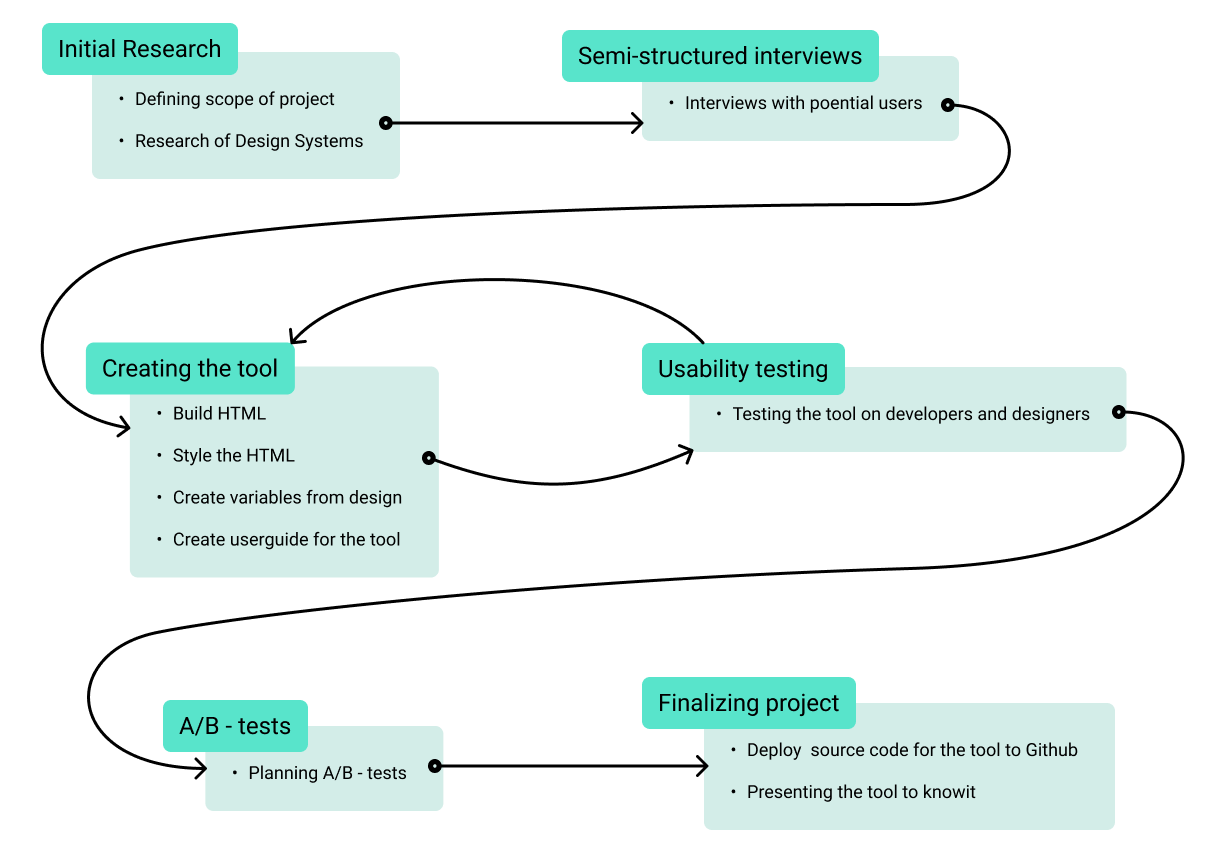
\includegraphics[width=\linewidth]{../images/Project flow chart.png}
  \caption{Flow chart over the project}
  \label{fig:projectFlowChart}
\end{figure}


\subsection{Initial Research}%
\label{sub:Initial Research}

At the start of the project, a meeting was held with a team at Knowit to determine their needs and their requirements on the project. After some discussion, there was an interest in creating an automated generating of code from their \acrshort{ui} design program, Figma. 

With this in mind, research began on what competitors there were in the field of code generation for web applications, and two competitors were most interesting, Webflow and Visly (see section \ref{sub:Competitors}). Some interesting small projects were also found that were used as inspiration for creating the tool. One project, especially creating color variables from Figma made by Karl Rombauts, was used \cite{rombautsKarlRombautsFigmaSCSSGenerator2021}.

How to encapsulate the Figma design elements into code was one of the most severe difficulties.  Different technologies were considered to find the fit for Knowit's requirements.  These technologies were using a JavaScript framework (such as Angular or React), plain \acrshort{html}-\acrshort{css}-JavaScript, or Web \glspl{component} with LitElement. 

One of the requirements was that the tool could be applicable for all types of projects. Using a JavaScript framework would mean that some projects would not support the tool. Therefore that technology was counted out. Using plain \acrshort{html}-\acrshort{css}-JavaScript could work for all projects, but it would be hard to manage since the generated code would be static and hard to encapsulate. Web \glspl{component} was chosen as the technology for encapsulating the Figma design elements into code. The lightweight JavaScript class LitElement was then chosen to make the creation of web components easier. LitElement is run natively in \acrshort{html}-\acrshort{css}-JavaScript, and therefore works with all projects. LitElement is also much easier to manage than just generating plain \acrshort{html}-\acrshort{css}-JavaScript.


% \begin{itemize}
%   \item Möte med knowit om behov och krav.
%   \item vad fanns för konkurrenter.
%   \item vilka liknande projekt fanns?
%   \item Vilka verktyg passade in knowits behov.

% \end{itemize}

\subsection{Semi-Structured Interviews}%
\label{sub:inteviews}
This tool is intended to be used by people in many different areas of expertise, from designers to front-end developers to back-end developers. A semi-structured interview model was used \cite{galletta2013mastering} to understand the work these people do in their respective roles to be able to build/develop a tool that is functional for all parts of the workflow (all the different roles in the workflow). The semi-structured interview was carried out with a script of questions that were asked to every interviewee. Unlike the structured interview, the semi-structured interview allows for further explanation and follow-up questions from the interviewer. These interviews were done with seven employees of Knowit Experience Umeå and Sundsvall. 

Because of the broad nature of the tool created, it was important to get participants that worked with all affected areas of expertise. The interviews were done digitally over Microsoft Teams \cite{VideoConferencingMeetings}. The scripts used for these interviews can be found in the appendix (The scripts are only in Swedish). 

\subsection{Creating the tool}%
\label{sub:creatingTool}
% After the interviews and research phase a clear understanding of the tools that would be used was had. (<--haha what) For creating the tool it self TypeScript was used to be able to use types to find problems before they crashed the code. LitElement was then used to 

The first step of creating the tool was discussing with Knowit what could be possible to achieve under the 20 week project time. As seen from the literature study, the big problem was how to condense the elements from the code to be used efficiently. 

The tool that was to be built would fetch data from Figmas \acrshort{rest}-\acrshort{api}, interpret the response from the \acrshort{api}, and build LitElement objects from the interpretation.

The tool was built using an experimental approach, meaning that code was tested, and possibilities were explored during the development of the program. TypeScript was chosen as the programming language because Knowit uses it in most projects and would therefore be familiar to them.

Figmas \acrshort{api} was examined to understand what was possible to do with it. Figmas website for developers\cite{figmaFigma} was read through and also some initial \acrshort{http}-requests were sent to the \acrshort{api}, using platform Postman \cite{PostmanCollaborationPlatform}. The initial response from the \acrshort{api} was large. This meant that setting the TypeScript types correct for all values in the response would be inefficient. To mitigate this the Visual Studio Code \cite{VisualStudioCode} extension quicktype\cite{ConvertJSONSwift} was used to generate types from the JSON response. 

From the \acrshort{api} response, we could see that most, or at least enough, of the data were the same as styling in \acrshort{css}. This meant that styling elements with \acrshort{css} were possible from the \acrshort{api}.

The information from Figmas \acrshort{api} was interpreted and stored as classes of colors, typographies, and \glspl{component}. The strategy was to generate a string that contained the LitElement. Essentially the program generated code as a string. This string is later written into a new TypeScript file that is then compiled into a JavaScript file that could be run in a browser.

\subsubsection{Building the HTML for the component}%
\label{ssub:building the skeleton of the component}
The Figma \glspl{component} have a parent-children structure, meaning that all \glspl{element} in the \gls{component} are related. A recursive function was used to search through each \gls{element} and their children dynamically. This replicates the relationship between the \glspl{element} and thereby creating a proper \acrshort{html} structure.

If the implementation of the before mentioned structure is not done correctly, the \glspl{element} would not be nested into each other.


\subsubsection{Styling the Component}%
\label{ssub:Styling the component}
One of the requirements from Knowit was that the \glspl{component} should be easy to alter. This meant that the style of the developer must be able to alter the style of the generated \gls{component}. 

In the first attempt to make this happen, all \acrshort{css} rules for an \gls{element} were assigned a \textit{property} in LitElement. A property allows the developer to pass data into the LitElement. By assigning a property for all \acrshort{css} rules of the \gls{element}, the style could be changed after generating the \gls{component}.

This was later redesigned because the user could not add \textit{new} \acrshort{css} rules to the component if they wished to. This problem was fixed by storing the \acrshort{css} rules in maps\cite{ArrayPrototypeMap} and pushing them into the correct \acrshort{css} selector. Instead of creating a property for each style attribute, only one property for each element is created. If the user wishes to add or change the styling of a component, they target the Figma element as an attribute to the component and inserts regular \acrshort{css}. The component then creates a duplicate of the styling map for the targeted element and inserts the new styling attributes into the component.


\subsubsection{Variables}%
\label{ssub:Variables}
Figma has a feature called styles. This is a way for the user to store and reuse colors, texts, and effects. This is something that is also very normal to do in a developer environment. Therefore a decision was made to create an \acrshort{scss} \textit{variable} file where these would be stored. Because of the time constraint of the project, only colors and texts were implemented. This was done similarly to the components where the ''code'' for the \acrshort{scss} variables was written to a string that later was written into an \acrshort{scss} file. 


\subsubsection{Open Source}%
\label{ssub:Open Source}
One of Knowit's initial requirements where that the software produced should be open source (see section \ref{ssub:Open Source}). The project was handed access to Knowit Experience Norrlands GitHub page. The software was uploaded publicly to this GitHub repository\cite{KnowitExperienceNorrlandFigmaConverter2021}. The MIT\cite{MITLicenseOpen} open source license where then attached to the repository stating that the software is free to use but has no liability or warranty.
 
\subsubsection{Userguide}%
\label{ssub:Userguide}
The program built does not have a graphical user interface, again because of the time constraint. The user is instead using a command-line interface (CLI). This makes it a bit harder to learn because there are no visual queues of what to input into the program.  A user guide was created in the form of a README on GitHub\cite{BuildSoftwareBetter} to solve this issue. Along side the prototype itself, this user guide was altered after the usability tests.

% knowit uses a supercharged version of css called scss in most of their projects (section \ref{sub:sass}). scss handles variables in a more intuitive way than regular  css which made it the clear choice for storing styling variables moving forward.




% \subsection{interviews from knowit}%
% \label{sub:}
% to get an understanding of what the tool should be able to do and how it should operate. semi-structured interviews were held with (??seven??) employees of knowit.





\subsection{Usability Testing}%
\label{sub:usertesting}
Usability tests were done to make sure that the prototype was usable for somebody else than the author. Furthermore, to set up the prototype for further testing regarding the effectiveness of the prototype.

Two iterations of usability testing were carried out on nine participants, four in the first iteration and five in the second iteration. The participants had to have a background in web development, \acrshort{npm}, and \acrshort{ui}-design software. Therefore, the participants chosen for the tests were employees of Knowit and students from the interaction and design program at the University of Umeå. The test was designed as a scenario with four different tasks. The participant first got a link to the GitHub repository where the prototype and the user guide were situated. The tasks were to create a viable Figma \gls{component} that could be converted to a web \gls{component} using the prototype. After that, the participant should install the prototype on their computer. Use the prototype to convert the Figma \gls{component} and then insert the \gls{component}, using \acrshort{npm} locally, in a test project supplied by the test administrator.

This was a way to test the whole chain from designing Figma \glspl{component}, converting these to web \glspl{component}, and to finally using the \glspl{component} in a project. These tests could also be used to determine what was working and not in the user guide. After the tasks were done, the questions about the experience were asked. Finally, the test administrator opened up for suggestions regarding improvements to the tool or the user guide. 

The test script was expanded in the second iteration to cover more features. These features were the use of color and text styles. The questions from the first iteration were still asked. This was done to confirm that the changes made between iteration one and iteration two were effective. 


\subsection{ A/B Testing }%
\label{sub:ab-testing}
To have a metric that can be measured, discussed, and statistically verifiable whether or not the prototype is effective in real-world use, A/B tests will be performed.  The primary goal of the test is the efficiency of the prototype. This will be an abnormal test, where instead of changing a small variable in an interface, the whole system will be tested. 

% The task for the participants of the test is to create a simple website from a description. The test participants will be working in pairs of designers and developers, where they ought to collaborate to complete the task. The task will be built using react, since 

% The ''control'' variant for the test will be creating a website as the participants are used to, and the ''challenger'' will be creating the website using the prototype. To establish a goal time to know when a test has passed. The ''control'' variant will be run multiple times to get an average time. This average time will then be used to signify the goal time. If the test is run faster than the goal time, it will pass. 

% The significance value for the test will be set to 95\%, meaning that the test will be performed until this value is met. 

The task for the participants of the test is to create a simple website from a description. The test participants will be working in pairs of designers and developers, where they ought to collaborate to complete the task. The participants would build the website using React.js since Knowit would use React.js for smaller projects.  

The A variant for the test would be building the website using React.js and the B variant using React.js and the prototype. The website would be built with a set of components. Then, a pilot test would be performed To understand how many and complicated these components should be.  This pilot test would be only on the A variant, where the description of the website would be changed according to how long each test took. The aim is to keep the tests under one hour to lower the fatigue of the test participants.

When the pilot testing is complete, an additional test would be performed where the A variant would be tested multiple times to get an average time. This average time would be set as the goal to beat for the A/B testing. If an A/B test is completed faster than the average time set from this A variant test, then the A/B test would ''pass''.  From this, we could determine a distribution of the ''passed'' test between variants A and B. Simulations would then be performed to get a significance value, that for this test would be 95\%. This means that a false positive occurs in every twenty tests, which could be considered high but is set for this initial test to try to save time.
